%%%%%%%%%%%%%%%%%%%%%%%%%%%%%%%%%%%%%%%%%
% Beamer Presentation
% LaTeX Template
% Version 1.0 (10/11/12)
%
% This template has been downloaded from:
% http://www.LaTeXTemplates.com
%
% License:
% CC BY-NC-SA 3.0 (http://creativecommons.org/licenses/by-nc-sa/3.0/)
%
%%%%%%%%%%%%%%%%%%%%%%%%%%%%%%%%%%%%%%%%%

%----------------------------------------------------------------------------------------
%	PACKAGES AND THEMES
%----------------------------------------------------------------------------------------

\documentclass{beamer}

\mode<presentation> {

% The Beamer class comes with a number of default slide themes
% which change the colors and layouts of slides. Below this is a list
% of all the themes, uncomment each in turn to see what they look like.

%\usetheme{default}
%\usetheme{AnnArbor}
%\usetheme{Antibes}
%\usetheme{Bergen}
%\usetheme{Berkeley}
%\usetheme{Berlin}
%\usetheme{Boadilla}
%\usetheme{CambridgeUS}
%\usetheme{Copenhagen}
%\usetheme{Darmstadt}
%\usetheme{Dresden}
%\usetheme{Frankfurt}
%\usetheme{Goettingen}
%\usetheme{Hannover}
%\usetheme{Ilmenau}
%\usetheme{JuanLesPins}
%\usetheme{Luebeck}
\usetheme{Madrid}
%\usetheme{Malmoe}
%\usetheme{Marburg}
%\usetheme{Montpellier}
%\usetheme{PaloAlto}
%\usetheme{Pittsburgh}
%\usetheme{Rochester}
%\usetheme{Singapore}
%\usetheme{Szeged}
%\usetheme{Warsaw}

% As well as themes, the Beamer class has a number of color themes
% for any slide theme. Uncomment each of these in turn to see how it
% changes the colors of your current slide theme.

%\usecolortheme{albatross}
%\usecolortheme{beaver}
%\usecolortheme{beetle}
%\usecolortheme{crane}
%\usecolortheme{dolphin}
%\usecolortheme{dove}
%\usecolortheme{fly}
%\usecolortheme{lily}
%\usecolortheme{orchid}
%\usecolortheme{rose}
%\usecolortheme{seagull}
%\usecolortheme{seahorse}
%\usecolortheme{whale}
%\usecolortheme{wolverine}

%\setbeamertemplate{footline} % To remove the footer line in all slides uncomment this line
%\setbeamertemplate{footline}[page number] % To replace the footer line in all slides with a simple slide count uncomment this line

%\setbeamertemplate{navigation symbols}{} % To remove the navigation symbols from the bottom of all slides uncomment this line
}

\usepackage{graphicx} % Allows including images
\usepackage{booktabs} % Allows the use of \toprule, \midrule and \bottomrule in tables

%----------------------------------------------------------------------------------------
%	TITLE PAGE
%----------------------------------------------------------------------
\begin{document}
\begin{frame}{Solving JEE 2008 GEOMETRY QUESTION USING MATRICES}
    

\title[Short title]{Solving JEE 2008 geometry question using matrices } % The short title appears at the bottom of every slide, the full title is only on the title page

\author{Rishitha\\Adithya} % Your name
\institute[UCLA] % Your institution as it will appear on the bottom of every slide, may be shorthand to save space

{Indian Institute of Technology Hyderabad \\ % Your institution for the title page
\medskip
\textit{ee18btech11033@iith.ac.in\\ee18btech11008@iith.ac.in} % Your email address
}
\date{\today} % Date, can be changed to a custom date
\end{frame}

\begin{frame}
\frametitle{Geometrical Question} 
A circle passes through two points (4,1) (6,5) and also the center lies on the equation 4x+y=16.Find the equation of the circle.
\end{frame}
\begin{frame}
\frametitle{Geometrical question in terms of matrices}
A circle passes through two points 
\begin{bmatrix}
4&1
\end{bmatrix}
,
\begin{bmatrix}
6&5
\end{bmatrix}
and also the center of the circle lies on the line 
\begin{bmatrix}
4&1
\end{bmatrix}
X=16 . Find the equation of the circle.
\end{frame}

%------------------------------------------------
\section{Diagram}

\section{Solution}

%------------------------------------------------

\begin{frame}
\frametitle{Solution}
Let A=\begin{bmatrix}
4\\1
\end{bmatrix} and B= \begin{bmatrix}
6\\5
\end{bmatrix}.Let the center of the circle be O.
The mid point of the chord AB is C =$\frac{A+B}{2}$=\begin{bmatrix}
5\\3
\end{bmatrix}
\newline Let the direction vector AB=B-A
\newline which gives AB=\begin{bmatrix}
2\\4
\end{bmatrix}
\newline The line joining C and O is normal to the chord AB. The equation of OC is:
\begin{equation}
    AB^T(x-C)=0
\end{equation}which gives
\centering
\begin{bmatrix}
2&4
\end{bmatrix}x=22
\end{frame}

%------------------------------------------------

\begin{frame}
\frametitle{Solution}
Given,the center of the circle also lies on line
\begin{bmatrix}
4&1
\end{bmatrix}X=16.
\newline\newlineThe center O is the point of intersection of OC and the given line.
\newline Let S =
\begin{bmatrix}
4&1\\2&4
\end{bmatrix} The point of intersection is given by:
\centering Sx=\begin{bmatrix}
16\\22
\end{bmatrix}.Then,
\begin{equation}
x=P^-^1b \end{equation}
\centering
x=$\frac{1}{14}$ \begin{bmatrix}
4&-1\\-2&4
\end{bmatrix}
\begin{bmatrix}
16\\22
\end{bmatrix}
\newline x= \begin{bmatrix}
3\\4
\end{bmatrix}
\end{frame}

%------------------------------------------------
\section{Second Section}
%------------------------------------------------
\begin{frame}
\frametitle{Solution}
The obtained Solution is nothing but the center..
\newline The radius can be obtained by computing the norm of (O-A) or (O-B)
\newline Radius = $||(O-B)||$=$||[3 - 1]||$=3.16 units
\newline Let o be the center of the circle.Then
\newline\centering $||x-c||$=r^2
\newline\begin{equation}
    (x-c)^T(x-c)=r^2\\
    x^Tx-2c^Tx=r^2-c^Tc\\
\newline \newline Therefore,the equation of the circle is given by,
\newline\newline x^Tx-2\begin{bmatrix}
    3&4
    \end{bmatrix}^Tx=3.16-\begin{bmatrix}
    3&4
    \end{bmatrix}^T\begin{bmatrix}
    3&4
    \end{bmatrix}
\end{equation}
\end{frame}
\begin{frame}{FIGURE}
\begin{figure}
    \centering
    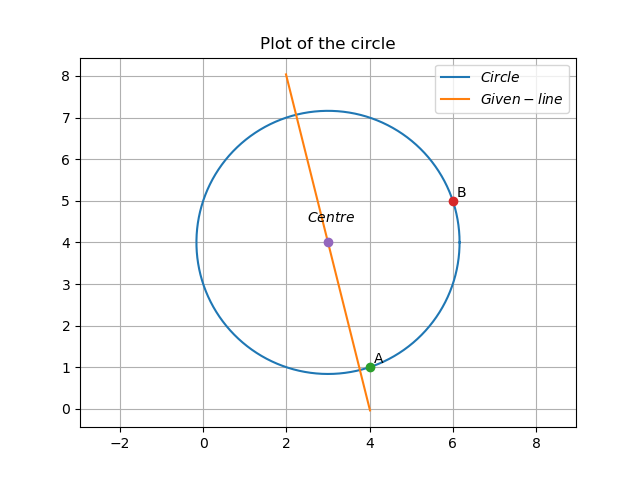
\includegraphics[scale=0.65]{Circle.png}
    \caption{Circle}
\end{figure}
\end{frame}
\end{document}